\documentclass[11pt]{article}
\PassOptionsToPackage{gray}{xcolor}
\usepackage{amsmath}
\usepackage[a4paper,margin=22mm]{geometry}
\usepackage{graphicx}
\usepackage{booktabs}
\usepackage{xcolor}
\usepackage{fontspec}
\usepackage[unicode,colorlinks=true,linkcolor=teal,urlcolor=teal]{hyperref}

\setmainfont[BoldFont=lmroman10-bold.otf]{lmroman10-regular.otf}
\definecolor{ReportInk}{HTML}{172B33}
\definecolor{ReportAccent}{HTML}{286C68}
\definecolor{ReportTint}{HTML}{EAF3F2}

\setlength{\parindent}{0pt}
\setlength{\parskip}{5pt}
\linespread{1.08}
\renewcommand{\arraystretch}{1.26}
\setlength{\tabcolsep}{5pt}

\newcommand{\reportlabel}[1]{{\large\color{ReportAccent}\bfseries #1}}
\newcommand{\reporttitle}[1]{%
  {\color{ReportInk}\Huge\bfseries #1\par}%
  \vspace{5mm}{\color{ReportAccent}\hrule height 1.3pt}%
}
\newcommand{\reportfigure}[3]{%
  \begin{center}
    {\bfseries #1}\par\smallskip
    \includegraphics[width=0.90\linewidth]{#2}\par\smallskip
    \begin{minipage}{0.9\linewidth}\small #3\end{minipage}
  \end{center}%
}

% Shared numeric values generated by python3 -m src.phase3_tables.
\newcommand{\PairedN}{843}
\newcommand{\StatusN}{1237}
\newcommand{\NormalN}{847}
\newcommand{\MissingScoreN}{4}
\newcommand{\ModelN}{842}
\newcommand{\ConfidencePct}{95}
\newcommand{\TestAlpha}{0.05}
\newcommand{\ThicknessCut}{2.319}
\newcommand{\HigherN}{486}
\newcommand{\LowerN}{357}
\newcommand{\TiedN}{3}
\newcommand{\Replicates}{10000}
\newcommand{\MeansSeed}{314159}
\newcommand{\ContrastSeed}{271828}
\newcommand{\MeanDF}{842}
\newcommand{\MeanCritical}{1.962785}
\newcommand{\DeltaEstimate}{0.3244}
\newcommand{\DeltaSE}{0.37616}
\newcommand{\DeltaT}{0.8624}
\newcommand{\DeltaDF}{786.6565}
\newcommand{\DeltaRawP}{0.38874}
\newcommand{\DeltaHolmP}{0.38874}
\newcommand{\DeltaLow}{-0.4140}
\newcommand{\DeltaHigh}{1.0628}
\newcommand{\DeltaWidth}{1.4768}
\newcommand{\DeltaBootMean}{0.3243}
\newcommand{\DeltaBootSE}{0.37306}
\newcommand{\DeltaBootLow}{-0.4119}
\newcommand{\DeltaBootHigh}{1.0489}
\newcommand{\DeltaBootWidth}{1.4608}
\newcommand{\DeltaWidthChange}{1.09}
\newcommand{\AnovaF}{40.4282}
\newcommand{\AnovaDFOne}{3}
\newcommand{\AnovaDFTwo}{28.7651}
\newcommand{\AnovaRawP}{\ensuremath{1.914\times10^{-10}}}
\newcommand{\AnovaHolmP}{\ensuremath{3.828\times10^{-10}}}
\newcommand{\EtaSquared}{0.1439}
\newcommand{\EtaPercent}{14.39}
\newcommand{\VarianceRatio}{4.159}
\newcommand{\SizeRatio}{121}
\newcommand{\ReviewCount}{11}
\newcommand{\ScoreMean}{22.3215}
\newcommand{\ScoreSD}{5.4350}
\newcommand{\ScoreSE}{0.18719}
\newcommand{\ScoreLow}{21.9541}
\newcommand{\ScoreHigh}{22.6889}
\newcommand{\ScoreBootSE}{0.18587}
\newcommand{\ScoreBootLow}{21.9561}
\newcommand{\ScoreBootHigh}{22.6821}
\newcommand{\ScoreWidthChange}{1.20}
\newcommand{\ThicknessMean}{2.336446}
\newcommand{\ThicknessSD}{0.121509}
\newcommand{\ThicknessSE}{0.004185}
\newcommand{\ThicknessLow}{2.328232}
\newcommand{\ThicknessHigh}{2.344660}
\newcommand{\ThicknessBootSE}{0.004185}
\newcommand{\ThicknessBootLow}{2.328230}
\newcommand{\ThicknessBootHigh}{2.344604}
\newcommand{\ThicknessWidthChange}{0.33}
\newcommand{\HigherScoreMean}{22.4588}
\newcommand{\HigherScoreSD}{5.5432}
\newcommand{\LowerScoreMean}{22.1345}
\newcommand{\LowerScoreSD}{5.2861}
\newcommand{\NormalGroupN}{847}
\newcommand{\NormalMean}{2.3364}
\newcommand{\NormalSD}{0.1213}
\newcommand{\NormalLow}{2.3282}
\newcommand{\NormalHigh}{2.3446}
\newcommand{\NormalSkew}{-0.950}
\newcommand{\NormalFlags}{15}
\newcommand{\ImpairedGroupN}{7}
\newcommand{\ImpairedMean}{2.3143}
\newcommand{\ImpairedSD}{0.1051}
\newcommand{\ImpairedLow}{2.2171}
\newcommand{\ImpairedHigh}{2.4115}
\newcommand{\ImpairedSkew}{-1.373}
\newcommand{\ImpairedFlags}{1}
\newcommand{\MCIGroupN}{252}
\newcommand{\MCIMean}{2.2576}
\newcommand{\MCISD}{0.1728}
\newcommand{\MCILow}{2.2361}
\newcommand{\MCIHigh}{2.2790}
\newcommand{\MCISkew}{-1.426}
\newcommand{\MCIFlags}{7}
\newcommand{\DementiaGroupN}{131}
\newcommand{\DementiaMean}{2.1541}
\newcommand{\DementiaSD}{0.2143}
\newcommand{\DementiaLow}{2.1170}
\newcommand{\DementiaHigh}{2.1911}
\newcommand{\DementiaSkew}{-0.556}
\newcommand{\DementiaFlags}{2}

\setmonofont{lmmono10-regular.otf}
\graphicspath{{figures/phase3/}}
\definecolor{ReportInk}{gray}{0}
\definecolor{ReportAccent}{gray}{0}
\definecolor{ReportTint}{gray}{0.95}
\hypersetup{pdftitle={Phase 3: Estimation and inference in the NACC teaching subset},allcolors=black,linkbordercolor={0 0 0},urlbordercolor={0 0 0}}
\newcommand{\numval}[1]{#1}
\newcommand{\ci}[2]{\ensuremath{[#1,\,#2]}}
\begin{document}
\reportlabel{Statistics course project, Track C (NACC)}\par
\vspace{5mm}
\reporttitle{Semantic verbal fluency and\\left inferior parietal cortical thickness}
{\Large Phase 3 | Sampling, estimation and inference\par}

\section{Question, participants and inferential plan}
Among participants with normal cognition, how does the mean number of
correct animal names in 60 seconds differ per 0.1 mm greater left inferior
parietal cortical thickness, after accounting for age, sex and education?
In Phase 3, we examine means and unadjusted group differences to build
toward this question. Phase 4 will estimate the adjusted continuous association.

Each supplied UDS and MRI file contains \StatusN{} unique participants.
We link the files one-to-one using NACCID. Every ID has a match, and
cognitive status agrees across the two files for everyone. Each person
contributes the single record supplied. The files do not give the source
number of visits, the index visit number, clinical or scan dates, or the
time between measurements. Participants are reported to have been selected
at random, but the sampling frame and selection probabilities are undocumented.

\begin{center}\small
\begin{tabular}{@{}p{0.72\linewidth}r@{}}
\toprule
Eligibility and use & People \\
\midrule
Usable UDS cognitive status and left MRI thickness; four-group comparison & \StatusN{} \\
Normal cognition before the score filter & \NormalN{} \\
Normal cognition with usable score and thickness; means and MRI-group contrast & \PairedN{} \\
Common eligible normal-cognition modeling sample, planned Phase 4 & \ModelN{} \\
\bottomrule
\end{tabular}
\end{center}

We exclude the \MissingScoreN{} unusable scores in the normal-cognition
group from score analyses. Thickness is finite and positive for every
matched participant. We follow the Phase 1 rules for excluding special
score codes and fractional counts, and retain all IQR-flagged measurements.
Passing these numerical checks does not establish scan quality. Details
of the source preparation and imputation are unknown.

Our target parameters describe the source population represented by this
extract, subject to each analysis's eligibility rules and sampling assumptions.
We assume that participants are independent. We set the plan after reviewing
the Phase 1 and 2 descriptions and before calculating the Phase 3 results;
the analyses are therefore exploratory. Individual intervals have
\ConfidencePct\% confidence. The two planned tests are a two-sided Welch
test of the MRI-group score difference and Welch one-way ANOVA of thickness
across cognitive groups. We use Holm adjustment to control their familywise
error rate at \TestAlpha{}.

\clearpage
\section{Two population means and their estimators}
For the same \PairedN{} eligible participants with normal cognition,
$\mu_A$ is the population mean animal-naming score and $\mu_T$ the
population mean left inferior parietal cortical thickness. Both are
estimated with the arithmetic sample mean, $\bar x=n^{-1}\sum_i x_i$.
Sample SD uses denominator $n-1$. The estimated standard error and
individual Student t interval are
\[
\widehat{\mathrm{SE}}(\bar x)=\frac{s}{\sqrt n},\qquad
\bar x\ \mathbin{\pm}\ t_{1-\alpha/2,n-1}\frac{s}{\sqrt n}.
\]
Here $n=\PairedN$, the degrees of freedom are \MeanDF{} and the
critical value is \MeanCritical{}.

\begin{center}\small
\begin{tabular}{@{}lrr@{}}
\toprule
Quantity & Animal-naming score & Left thickness (mm) \\
\midrule
Participants & \PairedN{} & \PairedN{} \\
Mean & \ScoreMean{} & \ThicknessMean{} \\
Sample SD & \ScoreSD{} & \ThicknessSD{} \\
Standard error & \ScoreSE{} & \ThicknessSE{} \\
Individual \ConfidencePct\% t interval & \ci{\ScoreLow}{\ScoreHigh} & \ci{\ThicknessLow}{\ThicknessHigh} \\
\bottomrule
\end{tabular}
\end{center}

The score counts correct responses in 60 seconds, while thickness is
measured in millimeters. The SD shows how much participants differ from
one another. The SE describes uncertainty in a mean estimated from
samples of this size. We interpret each SE in its own units because the
two measurements use different scales.

If we repeatedly sampled under the stated assumptions and built a nominal
95\% interval each time, about 95\% of those intervals would cover the
population parameter. This describes the interval procedure's coverage.
Once we observe the data, a particular interval has fixed endpoints.
It gives neither a posterior probability for the parameter nor the
range containing 95\% of individuals.

The t procedure has exact coverage for independent normal observations.
Here we use it as a large-sample approximation for the means. Its coverage
and the scope for generalization depend on the sampling assumptions.
Each interval concerns one parameter; we do not claim simultaneous 95\%
coverage for all reported parameters.

\clearpage
\section{Sampling distributions and empirical standard errors}
Using seed \MeansSeed{}, we draw \Replicates{} samples of \PairedN{}
complete participant rows with replacement. For each draw, we calculate
both means from the same rows so that each person's UDS and MRI measurements
stay together. The bootstrap SE is the sample SD of these replicate means,
calculated with denominator $B-1$.

\begin{center}\small
\begin{tabular}{@{}lrr@{}}
\toprule
Mean being estimated & Analytic SE & Bootstrap SE \\
\midrule
Animal-naming score (correct responses) & \ScoreSE{} & \ScoreBootSE{} \\
Left thickness (mm) & \ThicknessSE{} & \ThicknessBootSE{} \\
\bottomrule
\end{tabular}
\end{center}

\reportfigure{Figure 1. Sampling distribution of the score mean}{01_mean_score_sampling.pdf}{%
Each histogram value is a mean from one participant-level resample.
The dashed curve is a normal reference centered at the observed mean
with SD equal to its analytic SE. The solid line marks the observed mean;
the dotted limits are the individual 95\% bootstrap percentile interval.}

The resampled means cluster around the observed score mean. They vary
much less than individual scores because averaging \PairedN{} observations
reduces sampling variation. Resampling this extract gives an approximation
to a sampling distribution based on the observed values and the assumption
that participants are independent.

The small differences between analytic and bootstrap SEs have two sources:
the variance of the empirical distribution and Monte Carlo variation from
a finite number of replicates. Before that Monte Carlo approximation,
with-replacement resampling from the empirical distribution gives an exact
SE for the mean of $(s/\sqrt n)\sqrt{(n-1)/n}$. We retain all replicate
means in the numerical output.

\clearpage
\section{A bootstrap interval for the thickness mean}
The lower tail in individual thickness measurements gives us a reason
to compare the standard t interval with a bootstrap percentile interval.
We use the same participant resamples as for the score mean in Section 3.
After sorting the bootstrap means, we obtain the limits by linear
interpolation at rank $(B-1)p$, for $p=0.025$ and $p=0.975$.

\begin{center}\small
\begin{tabular}{@{}lcc@{}}
\toprule
Mean & Individual 95\% t interval & Individual 95\% percentile interval \\
\midrule
Score & \ci{\ScoreLow}{\ScoreHigh} & \ci{\ScoreBootLow}{\ScoreBootHigh} \\
Thickness (mm) & \ci{\ThicknessLow}{\ThicknessHigh} & \ci{\ThicknessBootLow}{\ThicknessBootHigh} \\
\bottomrule
\end{tabular}
\end{center}

\reportfigure{Figure 2. Sampling distribution of mean thickness}{02_mean_thickness_sampling.pdf}{%
The same \PairedN{} complete rows are drawn in each of \Replicates{}
replicates. The reference curve uses the analytic SE. Dotted limits show
the individual 95\% percentile interval, in millimeters.}

The thickness percentile interval is \ThicknessWidthChange\% narrower
than the t interval. Although individual measurements have a lower tail,
the resampled means are approximately bell-shaped at this sample size.
The two methods give similar uncertainty estimates for these data. This
agreement does not establish coverage in the population or count as an
independent replication.

\clearpage
\section{The MRI-group score contrast and first test}
For participants with normal cognition, we keep the Phase 2 pooled median
cutoff fixed at \ThicknessCut{} mm. The \TiedN{} paired participants whose
thickness equals the cutoff enter the higher group. Each person belongs
to just one MRI group, so the two groups contain different people and
we use an independent-samples comparison. Linking a person's UDS and MRI
records preserves their measurements together; it does not make this
between-group comparison paired.

\begin{center}\small
\begin{tabular}{@{}lrrr@{}}
\toprule
Left thickness group & People & Mean score & Sample SD \\
\midrule
At or above \ThicknessCut{} mm & \HigherN{} & \HigherScoreMean{} & \HigherScoreSD{} \\
Below \ThicknessCut{} mm & \LowerN{} & \LowerScoreMean{} & \LowerScoreSD{} \\
\bottomrule
\end{tabular}
\end{center}

The parameter is $\Delta=\mu_{A,H}-\mu_{A,L}$, in correct animal names
in 60 seconds. The registered hypotheses are $H_0:\Delta=0$ and
$H_1:\Delta\ne0$. The two-sided Welch method allows unequal group
sizes and variances. It uses
\[
\widehat{\mathrm{SE}}(\widehat\Delta)
=\sqrt{\frac{s_H^2}{n_H}+\frac{s_L^2}{n_L}},\qquad
T=\frac{\widehat\Delta}{\widehat{\mathrm{SE}}(\widehat\Delta)}
\]
with Welch--Satterthwaite degrees of freedom.

\begin{center}\small
\begin{tabular}{@{}lr@{}}
\toprule
Quantity & Result \\
\midrule
Higher-minus-lower mean difference & \DeltaEstimate{} \\
SE of the difference & \DeltaSE{} \\
Welch t statistic; degrees of freedom & \DeltaT{}; \DeltaDF{} \\
Individual 95\% Welch interval & \ci{\DeltaLow}{\DeltaHigh} \\
Raw p-value; Holm-adjusted p-value & \DeltaRawP{}; \DeltaHolmP{} \\
\bottomrule
\end{tabular}
\end{center}

If the population mean difference were zero and the Welch assumptions
held, the approximate probability of an absolute t statistic at least
as large as \DeltaT{} would be \DeltaRawP{}. At familywise level
\TestAlpha{}, we therefore have insufficient evidence of a mean score
difference. The interval includes zero and differences in either
direction. We have not specified a meaningful equivalence margin, so
this result cannot establish equality or practical equivalence.

\clearpage
\section{Participant-level bootstrap of the score difference}
Using seed \ContrastSeed{}, we generate \Replicates{} replicates. Each
replicate resamples \HigherN{} complete participant rows with replacement from the
higher MRI group and \LowerN{} from the lower group. The groups are
resampled independently, drawing the higher group first and the lower
group second from one local random stream. We keep the group sizes,
cutoff and subtraction direction fixed, and keep each person's UDS and
MRI measurements together.

\begin{center}\small
\begin{tabular}{@{}lccc@{}}
\toprule
Method & SE & Individual 95\% interval & Width \\
\midrule
Welch & \DeltaSE{} & \ci{\DeltaLow}{\DeltaHigh} & \DeltaWidth{} \\
Bootstrap percentile & \DeltaBootSE{} & \ci{\DeltaBootLow}{\DeltaBootHigh} & \DeltaBootWidth{} \\
\bottomrule
\end{tabular}
\end{center}

\reportfigure{Figure 3. Resampled score differences and interval comparison}{03_score_difference_bootstrap.pdf}{%
The histogram summarizes higher-minus-lower differences from the fixed-size
group resamples. The lower panel compares individual 95\% intervals.
Each point marks the same observed difference, \DeltaEstimate{} correct responses.}

The bootstrap interval is \DeltaWidthChange\% narrower. The resampled
differences average \DeltaBootMean{}, close to the observed difference,
and both intervals include zero. This bootstrap distribution describes
uncertainty around the observed effect. It is not a null distribution
for calculating another p-value. We assess practical importance using
the raw difference and its interval in correct responses. This comparison
remains exploratory and does not adjust for covariates.

\clearpage
\section{Thickness across UDS cognitive groups and second test}
For the supplementary cross-modal comparison, we group MRI thickness
by UDS cognitive status in all \StatusN{} eligible participants. The
normal-cognition group contains \NormalN{} people here because this
comparison does not require a usable score. We test
$H_0:\mu_1=\mu_2=\mu_3=\mu_4$ against the alternative that at least
one mean differs.

\begin{center}\small
\begin{tabular}{@{}lrrc@{}}
\toprule
Cognitive status & People & Mean (mm) & Individual 95\% t interval (mm) \\
\midrule
Normal cognition & \NormalGroupN{} & \NormalMean{} & \ci{\NormalLow}{\NormalHigh} \\
Impaired without MCI & \ImpairedGroupN{} & \ImpairedMean{} & \ci{\ImpairedLow}{\ImpairedHigh} \\
MCI & \MCIGroupN{} & \MCIMean{} & \ci{\MCILow}{\MCIHigh} \\
Dementia & \DementiaGroupN{} & \DementiaMean{} & \ci{\DementiaLow}{\DementiaHigh} \\
\bottomrule
\end{tabular}
\end{center}

Welch ANOVA gives $F=\AnovaF$ with degrees of freedom
$(\AnovaDFOne,\AnovaDFTwo)$, raw p = \AnovaRawP{} and Holm-adjusted
p = \AnovaHolmP{}. The method allows unequal variances. If all four
population means were equal and the assumptions held, the raw p-value
would be the approximate probability of an F statistic at least as
large as \AnovaF{}.

\reportfigure{Figure 4. Group means and their precision}{04_thickness_group_means.pdf}{%
Points show mean thickness; bars show individual 95\% t intervals. The
seven-person group's wide interval makes its limited precision visible.
These intervals do not constitute adjusted pairwise comparisons.}

The descriptive sample eta-squared is \EtaSquared{}, calculated as
between-group SS divided by total SS. About \EtaPercent\% of the observed
squared thickness variation lies between group means. This summary
depends on the sample composition and is separate from the precision
weights used in the Welch F statistic. Under the model, the omnibus test
supports a difference in at least one mean. It does not tell us which
pair of means differs.

\clearpage
\section{Distribution and assumption checks}
The largest group is \SizeRatio{} times the size of the smallest, and
the largest sample variance is \VarianceRatio{} times the smallest.
Alongside the test, we examine group sizes, SDs, ranges, quartiles,
tail asymmetry and IQR flags. Welch allows unequal variances and group
sizes, but the accuracy of its approximation still depends on the
distributions, especially in a small group.

\begin{center}\small
\begin{tabular}{@{}lrrr@{}}
\toprule
Cognitive status & Sample SD (mm) & Empirical skewness & IQR flags retained \\
\midrule
Normal cognition & \NormalSD{} & \NormalSkew{} & \NormalFlags{} \\
Impaired without MCI & \ImpairedSD{} & \ImpairedSkew{} & \ImpairedFlags{} \\
MCI & \MCISD{} & \MCISkew{} & \MCIFlags{} \\
Dementia & \DementiaSD{} & \DementiaSkew{} & \DementiaFlags{} \\
\bottomrule
\end{tabular}
\end{center}

\begin{center}
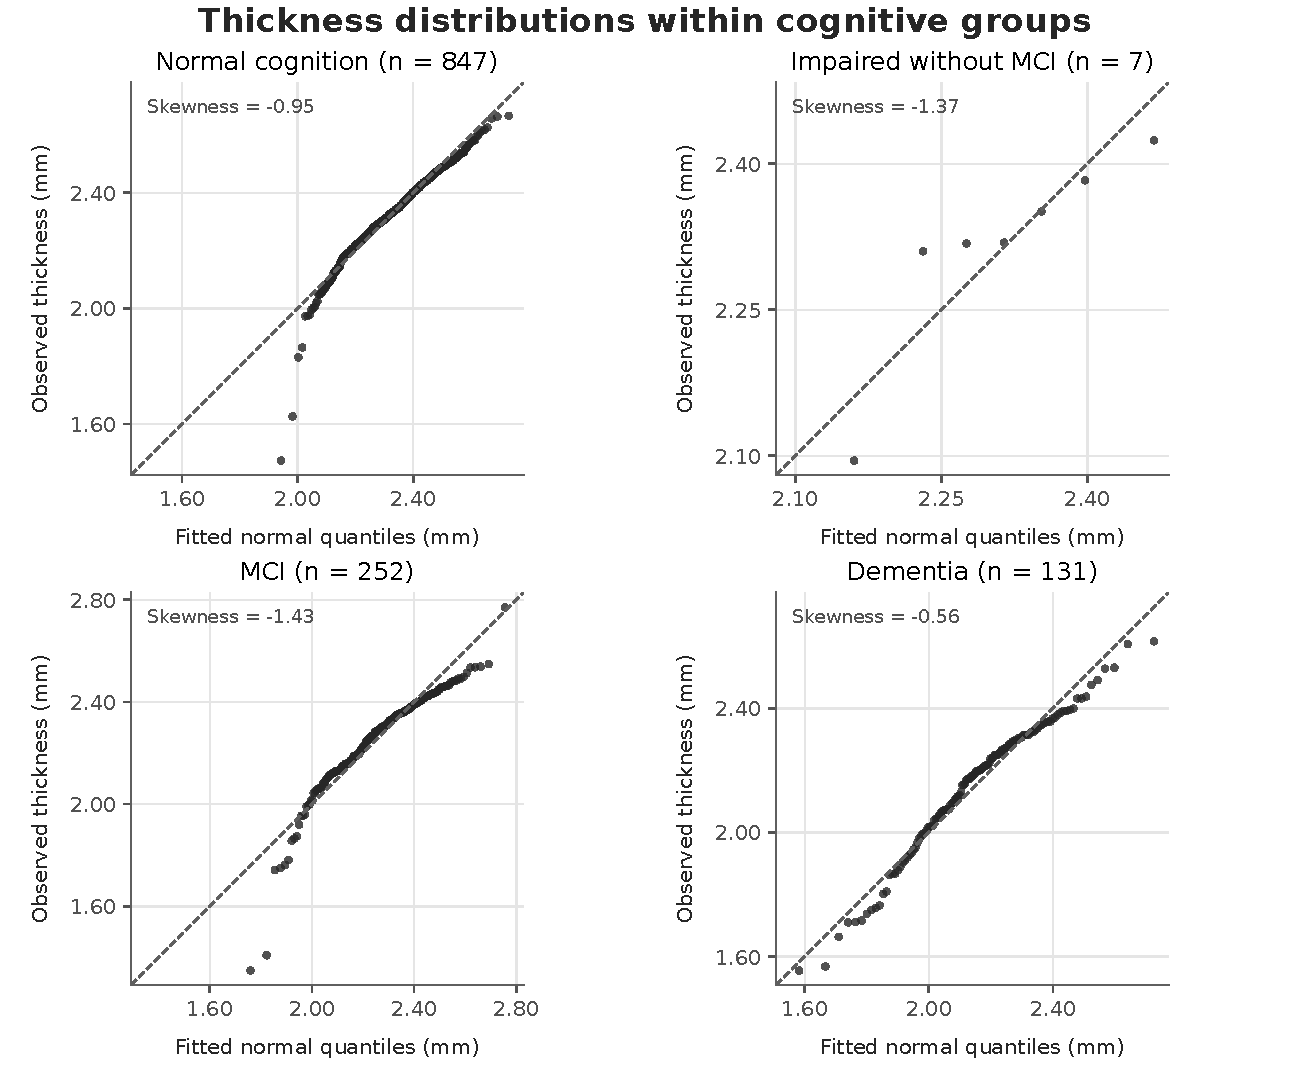
\includegraphics[width=0.99\linewidth]{05_thickness_group_qq.pdf}\par
\begin{minipage}{0.96\linewidth}\small
\textbf{Figure 5. Within-group normal Q-Q checks.} Every participant is
shown, including all seven observations in the smallest group. The
reference line compares observed quantiles with a fitted normal distribution.
\end{minipage}
\end{center}

The lower tails depart from the normal reference. The group classified
as impaired without MCI has only seven people, including a low-tail
observation. Its mean interval and the Welch approximation are sensitive
to non-normality and individual extreme values. We retain all flagged
measurements and interpret the result as an exploratory comparison under
the model. Agreement between calculations cannot validate the
distributional assumptions.

\clearpage
\section{Completed test family and integrated interpretation}
We use Holm adjustment to control the planned family of two tests at
$\alpha=\TestAlpha$, provided the raw p-values are valid. The procedure
sorts the raw p-values, multiplies each by the number of tests remaining,
takes cumulative maxima and caps the results at one. It also allows
dependence between tests. The completed table gives the final adjusted
values; earlier step files keep the status recorded at those stages.

\begin{center}\small
\begin{tabular}{@{}p{0.44\linewidth}ccc@{}}
\toprule
Planned comparison & Raw p & Holm p & Reject after Holm? \\
\midrule
Score in two MRI groups, normal cognition & \DeltaRawP{} & \DeltaHolmP{} & No \\
Thickness in four cognitive groups & \AnovaRawP{} & \AnovaHolmP{} & Yes \\
\bottomrule
\end{tabular}
\end{center}

Within normal cognition, the grouped score comparison leaves both the
size and direction of the difference uncertain. Across cognitive statuses,
the omnibus MRI comparison gives evidence of a difference in at least
one mean, subject to the method's assumptions. These results concern
different parameters and eligibility samples. Phase 4 will address the
primary continuous association per 0.1 mm, adjusting for age, sex and
education in the common \ModelN{}-person eligible sample.

We read p-values alongside effects in their original units and the widths
of their intervals. A p-value is not the probability that the null
hypothesis is true, and statistical significance alone does not establish
practical importance. No practical equivalence margin has been supplied.
The group mean intervals are individual intervals, and the omnibus result
alone cannot establish significance for a selected pair of groups.

The sampling frame, source preparation and imputation methods are
undocumented, and we have no masks identifying which values were imputed.
Our estimates and resampling therefore condition on the supplied values;
these files cannot tell us how much extra uncertainty preparation adds.
Clinical/MRI timing and scan-level QC are also unavailable. Having one
record per ID confirms the input structure, while independence across
people remains a model assumption. The small, skewed group and unknown
sampling design limit the accuracy of inference and its generalizability.
These exploratory observational results describe associations under the
stated eligibility rules and do not establish causation.

\clearpage
\section{Reproducibility, requirement coverage and sources}
We generate the report's numbers with \texttt{src.phase3\_tables}
from the verified JSON results. The notebook runs the calculations and
checks them against the saved outputs. The integrated review passed
\ReviewCount{} consistency checks: rebuilding from raw CSVs, checking
fixed sample rules and retained bootstrap draws, verifying the test family,
and exactly reproducing all five grayscale vector figures. The review file
\texttt{reports/phase3/inference\_review.json}
records source hashes and environment versions.

After the shared analysis, the final review and table-generation steps are
\begin{verbatim}
python3 -m src.phase3_review
python3 -m src.phase3_tables
\end{verbatim}
The README gives the full sequence of analysis commands,
LaTeX builds and notebook execution instructions. Raw participant CSVs
stay local. The student handles Git publication, the phase-3 tag and
CW packaging manually.

\begin{center}\small
\begin{tabular}{@{}p{0.19\linewidth}p{0.73\linewidth}@{}}
\toprule
Course requirement & Evidence in this report \\
\midrule
General 1; C2 & Section 2 defines two population means, estimators, units and intervals. \\
General 2 & Sections 3--4 show resampled means and compare empirical and analytic SEs. \\
General 3 & Section 2 gives mean intervals and their repeated-sampling interpretation. \\
General 4; C3 & Section 5 compares independent MRI groups using a score-difference interval. \\
General 5 & Sections 1, 5 and 7 specify hypotheses, methods, assumptions and the test family. \\
General 6 & Sections 5, 7 and 9 interpret raw and adjusted p-values in context. \\
General 7; C5 & Sections 4 and 6 compare standard and percentile intervals; whole rows are resampled. \\
General 8; C4 & Sections 7--8 give Welch ANOVA and distribution/assumption diagnostics. \\
General 9 & Sections 5, 7 and 9 report raw effects, sample eta-squared and practical limits. \\
C1 & Section 1 documents one supplied record per participant and ID-based linkage. \\
\bottomrule
\end{tabular}
\end{center}

{\small
\textbf{Sources.} Statistics course project guide, pp. 4--5, 10--13 and
18--19; NACC teaching extract and data dictionaries documented in the
project card. Methods follow the official SciPy documentation for
\href{https://docs.scipy.org/doc/scipy/reference/generated/scipy.stats.ttest_ind.html}{Welch t testing},
\href{https://docs.scipy.org/doc/scipy/reference/generated/scipy.stats.bootstrap.html}{bootstrap SEs and percentile intervals}, and
\href{https://docs.scipy.org/doc/scipy/reference/generated/scipy.stats.f_oneway.html}{Welch ANOVA}.
\href{https://stat.ethz.ch/R-manual/R-devel/library/stats/html/p.adjust.html}{R's p.adjust documentation}
describes Holm control; the
\href{https://www.amstat.org/asa/files/pdfs/P-ValueStatement.pdf}{ASA statement on p-values}
informs interpretation. All URLs are linked in the PDF.\par}
\end{document}
